\section{Results}\label{art.res}
Results of model calibration and inferred dynamics of heterosexual HIV transmission in Eswatini
are given in \sref{model.res}~and~\ref{app.model.cal.res}.
This section focuses on results of scenarios and analyses outlined in \sref{art.meth.obj}.
%===================================================================================================
\subsection{Objective~1: Influence of cascade differences between risk groups}\label{art.res.1}
Figure~\ref{fig:art.1.cascade} illustrates cascade attainment over time
in each of the four counterfactual scenarios (\casmd overall by 2020),
plus the base case (\cashi overall by 2020).
Figure~\ref{fig:art.1.rai} then illustrates
cumulative additional infections (CAI) and additional incidence rate (AIR)
in each counterfactual scenario \vs the base case.
Leaving behind both FSW and clients resulted the most additional infections: median [IQR]
28.8~[17.5,~46.2]\,\% more than the base case by 2030. % MAN
By contrast, leaving behind neither FSW nor clients resulted in the fewest additional infections:
13.0~[6.1,~25.6]\,\% more than the base case by 2030 --- % MAN
a 54.2~[30.3,~73.2]\,\% reduction. % MAN TODO: (!)
Leaving behind either FSW or clients resulted in a similar number of additional infections:
21.8~[12.5,~36.7]\,\% and 20.4~[11.8,~34.7]\,\%, respectively. % MAN
Relative differences were similar for additional incidence rate.
Which risk groups acquired additional infections differed across scenarios
(Figure~\ref{fig:art.1.wiw.to}),
with more additional infections among clients when FSW were left behind,
\vs among lower risk risk women when clients were left behind.
The majority of additional infections were transmitted
via casual partnerships in all scenarios (Figure~\ref{fig:art.1.wiw.part}). % MAN
\begin{figure}[h]
  \centering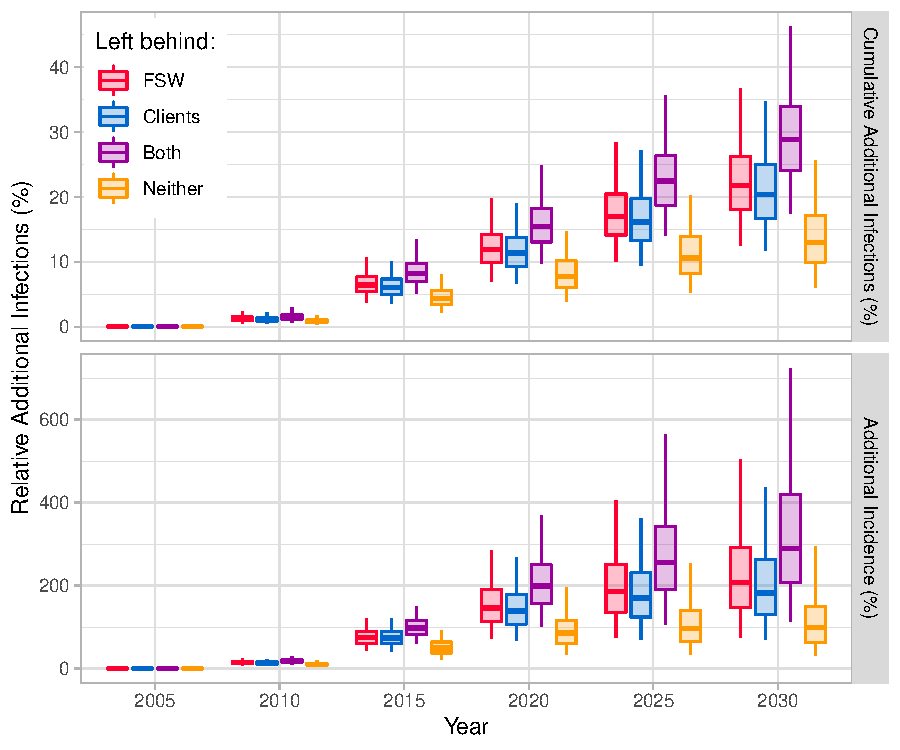
\includegraphics[width=.8\linewidth]{art.1.rai}
  \caption{Relative additional infections under counterfactual scenarios \vs the base case}
  \label{fig:art.1.rai}
  \floatfoot{\ffart; \ffbox.}
\end{figure}
%===================================================================================================
\subsection{Objective~2: Conditions under which cascade differences matter most}\label{art.res.2}
The fitted regression models \eqref{eq:art.glm} indicated that
population-overall viral unsuppression ($D$) and
group-specific unsuppression among FSW and clients ($d_i$)
were each strongly and positively associated with the CAI and AIR outcomes ($p < 10^{-5}$).
These associations support the results of Objective~\ref{obj:art.1}.
Figure~\ref{fig:art.2} plots the estimated effects of
group-specific unsuppression $d_i$, and
effect modification by epidemic conditions $C_j$.
The effect of unsuppression among FSW on CAI increased with:
FSW and client population sizes, client turnover, and
HIV incidence ratio among FSW \vs other women.
The effect of unsuppression among clients on CAI increased with:
FSW and client population sizes and FSW turnover.
Effect modification results for AIR were similar to CAI among both FSW and clients.
\begin{figure}[h]
  \subcapoverlap\centering
  \foreach \var in {cai,air}{\vskip1ex
    \begin{subfigure}{.75\linewidth}
      \includegraphics[width=\linewidth]{art.2.\var}
      \caption{\raggedright}
      \label{fig:art.2.\var}
    \end{subfigure}}
  \caption{}
  \label{fig:art.2}
  \floatfoot[.75]{
  \ffpbar{effect}.}
\end{figure}
\pagebreak % TEMP
